% !TEX program = pdflatex   % ← 能编译，但内容仍有8个格式错误
\documentclass[12pt,a4paper]{ctexart}

\usepackage[top=2.5cm, bottom=2.5cm, left=3.0cm, right=2.5cm]{geometry}
\usepackage{setspace}
\onehalfspacing
\usepackage{times}

% ← 错误1：手动指定字体（多余，ctex自动处理）
\setCJKmainfont{SimSun}
\setCJKsansfont{SimHei}
\setCJKmonofont{KaiTi}

\usepackage{graphicx}
\usepackage{caption}
\usepackage[colorlinks=true]{hyperref}

% ← 错误2：无页眉页脚设置（缺少 fancyhdr）

\begin{document}

% ========== 封面 ==========
% ← 错误3：多了大标题
\begin{center}
    {\heiti\zihao{1} 江苏大学课程论文}
    
    \vspace{2cm}
    
    {\heiti\zihao{3} 太阳能光伏发电技术综述}
    
    \vspace{3cm}
    
    {\songti\zihao{4}
    专业班级：微电子2201\hspace{3em}学生姓名：超级老付
    
    \vspace{0.5cm}
    
    指导教师：李四\hspace{4.5em}职\quad 称：教授   % ← 错误4：职称应为讲师
    
    \vspace{2cm}
    
    日\quad 期：2026年6月1日   % ← 错误5：不应有日期
    }
\end{center}

% ========== 原创性声明 ==========
% ← 错误6：不应有此声明
\newpage
\begin{center}
    {\heiti\zihao{3} 原创性声明}
\end{center}
本人郑重声明：所呈交的课程论文，是本人在指导教师指导下独立完成的成果。\par
\hspace{2em}论文作者签名：\hspace{2cm}日 期：\hspace{2cm}

\newpage

% ========== 中文摘要 ==========
\begin{center}
    {\heiti\zihao{4} 摘\quad 要}
\end{center}

太阳能光伏发电是新能源领域的重要方向。本文综述了光伏技术的发展现状\cite{ref1}，分析其应用前景。

\vspace{12bp}
\noindent{\heiti 关键词：} 光伏发电；新能源；可再生能源

% ========== 英文摘要 ==========
% ← 错误7：不应有英文摘要
\newpage
\begin{center}
    {\bfseries\zihao{4} Abstract}
\end{center}

Solar photovoltaic power generation is an important direction in the field of new energy. This paper reviews the current status of photovoltaic technology\cite{ref1}.

\vspace{12bp}
\noindent{\bfseries Keywords:} Photovoltaic; New Energy; Renewable Energy

\newpage
\tableofcontents
\newpage

% ========== 正文 ==========
\section{引言}

随着全球能源转型加速，太阳能光伏发电技术受到广泛关注\cite{ref1}。近年来，光伏电池效率不断提升，成本持续下降\cite{ref2}。

\section{光伏技术分析}
光伏技术主要包括晶硅电池、薄膜电池和钙钛矿电池三大类。

\begin{center}
    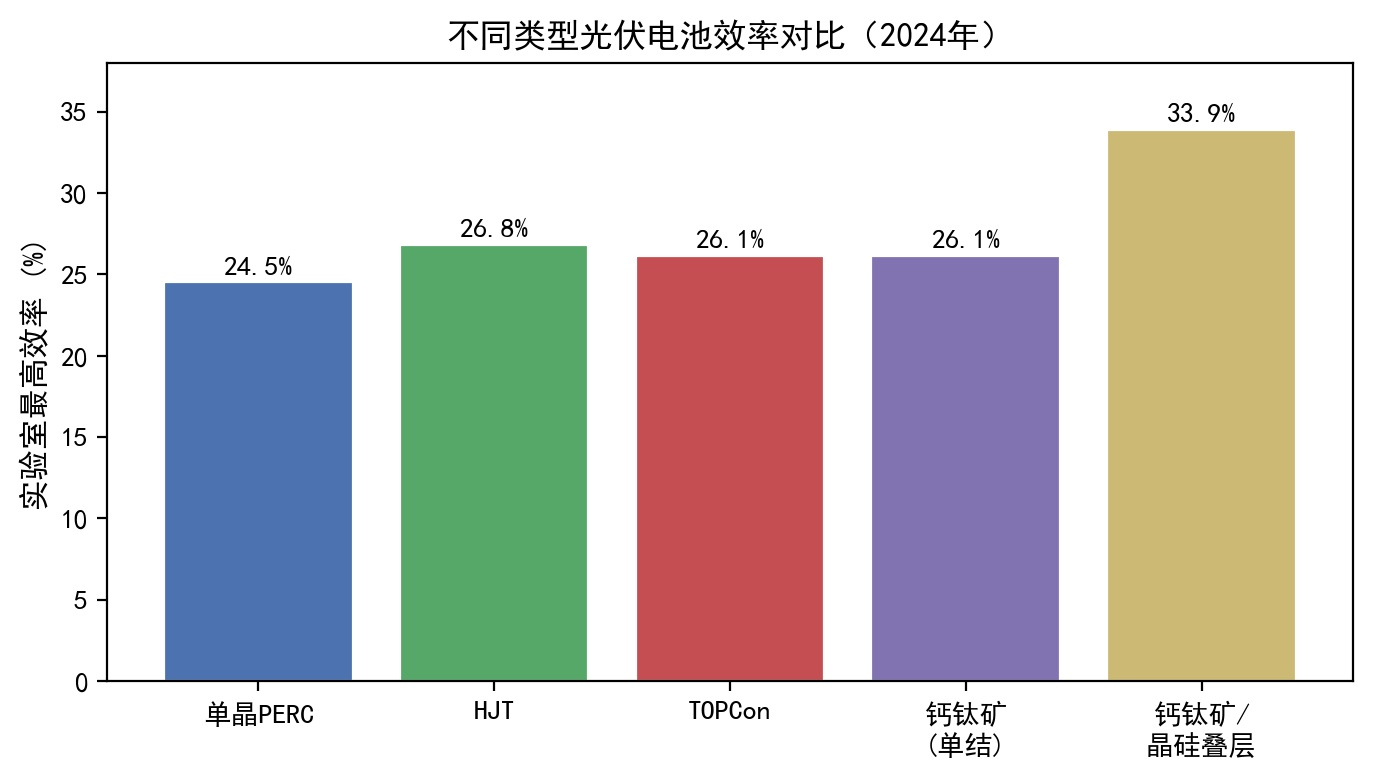
\includegraphics[width=0.7\textwidth]{figures/demo_chart.jpg}
    \captionof{figure}{光伏电池效率对比}
\end{center}

\section{应用现状}
光伏发电已在全球大规模部署，2024年全球累计装机容量超过1TW。

\section{结论与展望}
本文综述了光伏技术现状和趋势\cite{ref2}。未来钙钛矿叠层电池有望突破30\%效率\cite{ref1}。

% ← 错误8：结论中有引用

\newpage
% ← 错误9：参考文献缺页眉页脚设置
\begin{thebibliography}{99}
\bibitem{ref1} 张三, 李四. 太阳能电池技术进展[J]. 物理学报, 2023, 72(5): 1-15.
\bibitem{ref2} 王五. 光伏发电系统设计[M]. 北京: 科学出版社, 2022.
\end{thebibliography}

\end{document}
